\chapter{Datasets statistics}

\begin{figure}[hbt]
  \centering
  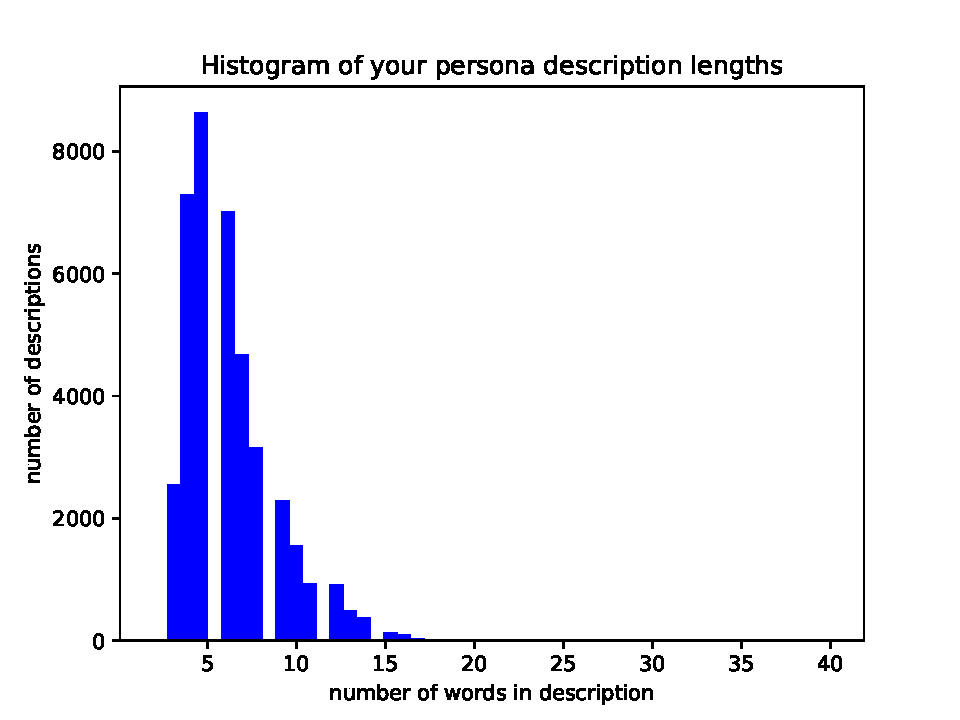
\includegraphics[width=0.7\textwidth]{figures/persona_desc.pdf}
  \caption{Histogram of persona description lengths.}
  \label{fig:histogram_persona_desc}
\end{figure}

\begin{figure}[hbt]
  \centering
  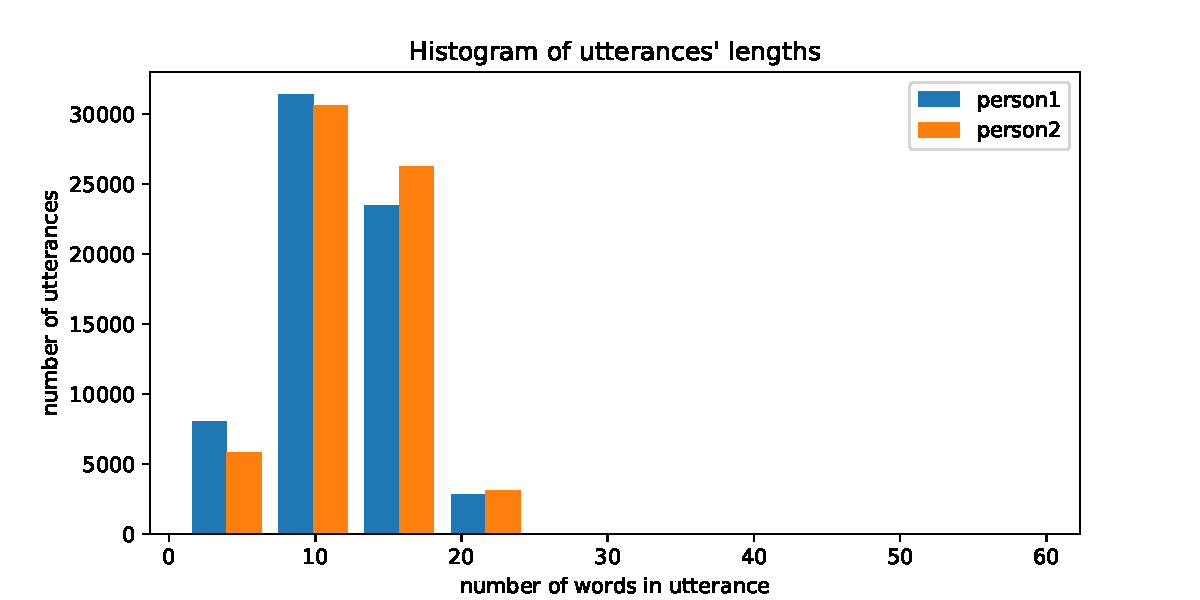
\includegraphics[width=0.7\textwidth]{figures/uttr_length.pdf}
  \caption{Histogram of utterances' lengths of a person.}
  \label{fig:histogram_uttr_length}
\end{figure}

\begin{figure}
  \centering
  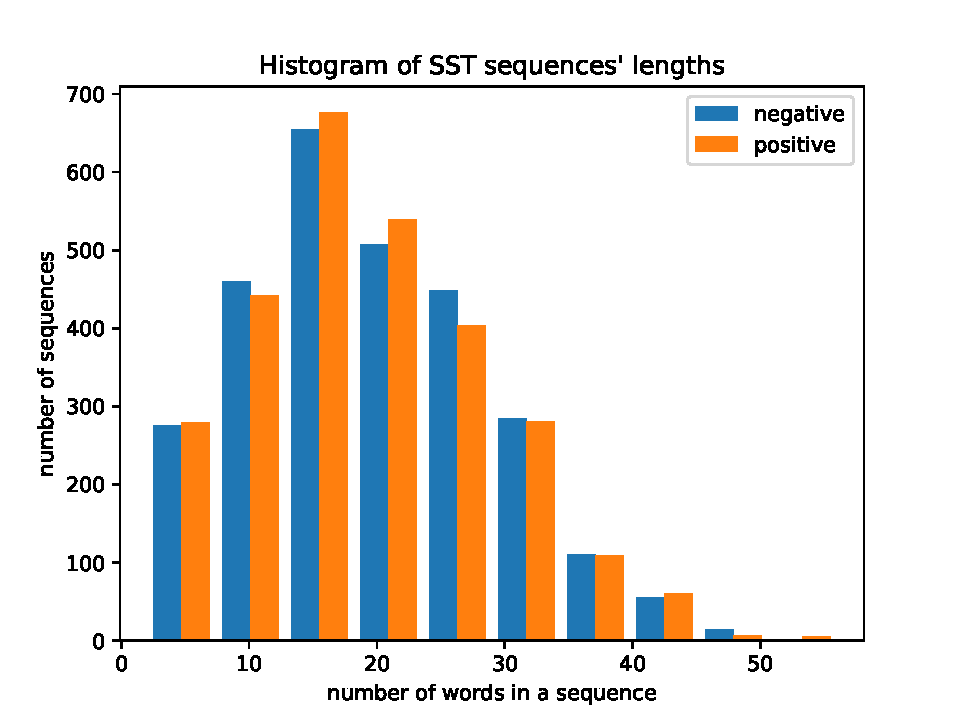
\includegraphics[width=0.7\textwidth]{figures/sst.pdf}
  \caption{Histogram of Stanford Sentiment Treebank labeled reviews.}
  \label{fig:sst}
\end{figure}

\begin{figure}
  \centering
  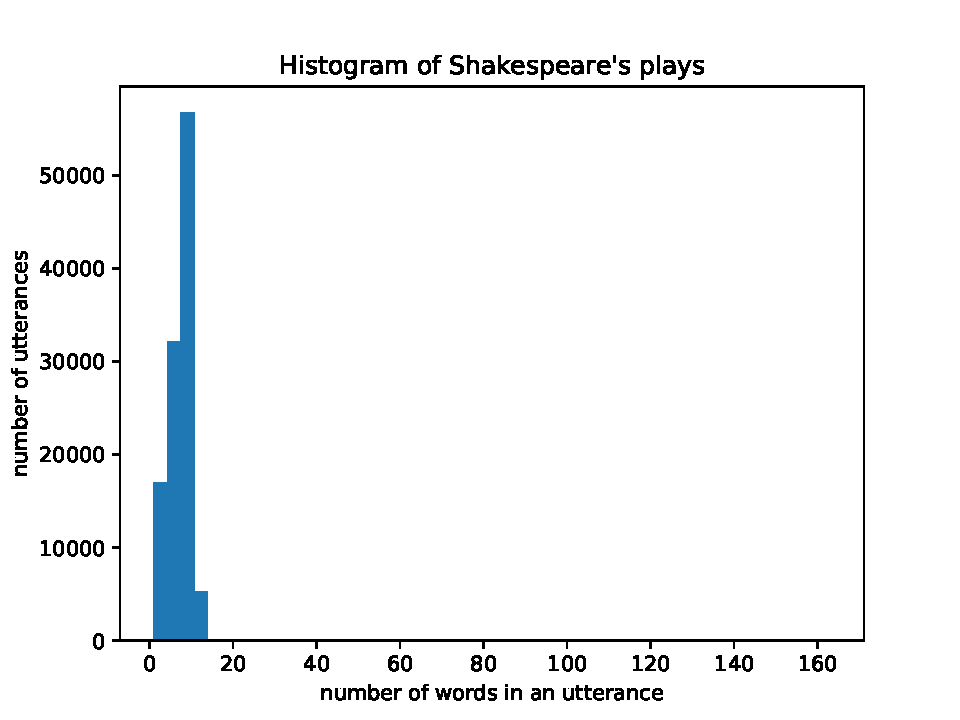
\includegraphics[width=0.7\textwidth]{figures/shakespeare.pdf}
  \caption{Histogram of Shakespeare's plays.}
  \label{fig:shakespeare}
\end{figure}

\begin{figure}[hbt]
  \centering
  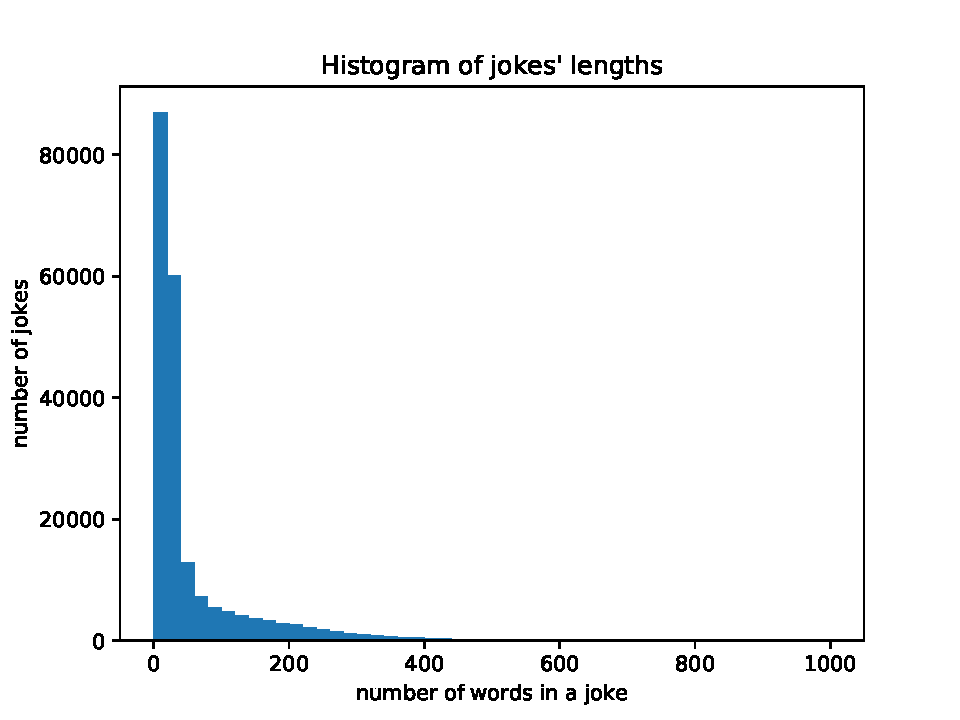
\includegraphics[width=0.7\textwidth]{figures/jokes.pdf}
  \caption{Histogram of jokes lengths.}
  \label{fig:jokes}
\end{figure}

\begin{figure}[hbt]
  \centering
  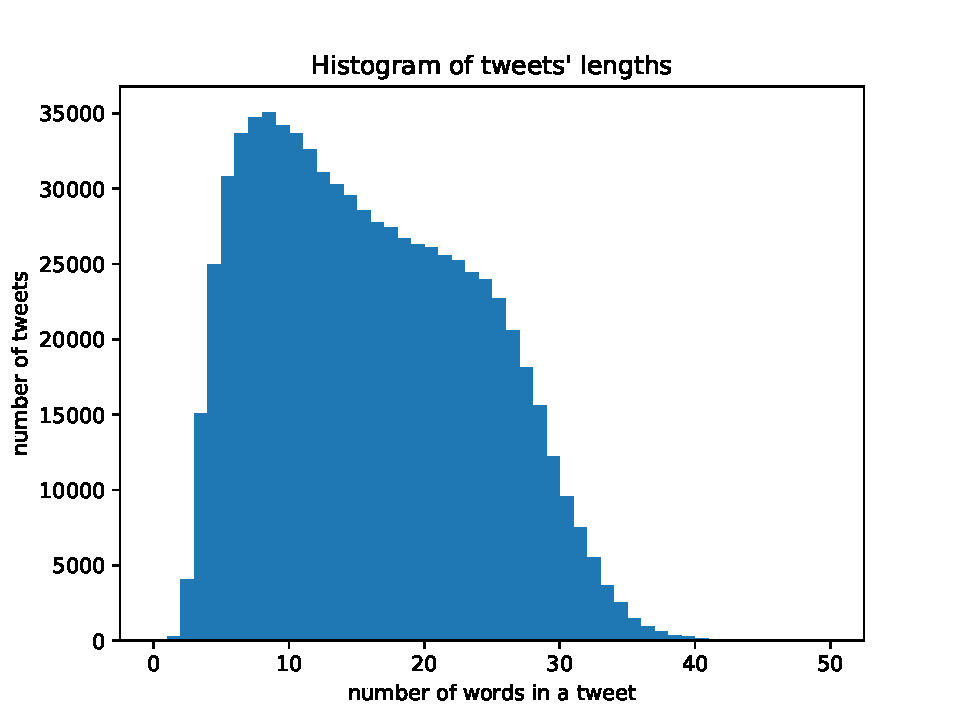
\includegraphics[width=0.7\textwidth]{figures/tweet.pdf}
  \caption{Histogram of tweets' lengths.}
  \label{fig:tweet}
\end{figure}

\chapter{Examples of experiments}

\begin{table}[ht]
\centering
 \begin{tabular}{|p{14cm}|}
 \hline\hline
 \textbf{Person 1 description:} 1. as a child, i won a national spelling bee. 2. i have been published in the new yorker magazine. 3. i am a gourmet cook. 4. i have perfect pitch. \\
 \hline
 \textbf{Person 2 description:} 1. i am very athletic. 2. i wear contacts. 3. i have brown hair. 4. i love bicycling. 5. i hate carrots. \\
 \hline\hline
 \textbf{Person1:} i am afraid. \\
 \textbf{Person2:} i am a business employee.  \\ 
 \textbf{Person1:} i am a surfer. \\
 \textbf{Person2:} i am not much of a foodie. \\
 \textbf{Person1:} i am afraid. \\
 \textbf{Person2:} that is cool. \\
 \textbf{Person1:} i do. i like to starve. \\
 \textbf{Person2:} i like to go to the homeless. \\
 \textbf{Person1:} i am not really a fan of harry potter. \\
 \textbf{Person2:} i am good. i am in tampa. \\
 \textbf{Person1:} i am from boston ma. \\
 \textbf{Person2:} i am in boston. \\
 \hline\hline
 \end{tabular}
 \caption{Example of a dialogue conversation generated by baseline model.}
\label{tab:baseline_experiment}
\end{table}

\begin{table}[ht]
\centering
 \begin{tabular}{|p{14cm}|}
 \hline\hline
 \textbf{Person 1 description:} 1. as a child, i won a national spelling bee. 2. i have been published in the new yorker magazine. 3. i am a gourmet cook. 4. i have perfect pitch. \\
 \hline
 \textbf{Person 2 description:} 1. i am very athletic. 2. i wear contacts. 3. i have brown hair. 4. i love bicycling. 5. i hate carrots. \\
 \hline\hline
 \textbf{Person1:} hi, how are you doing today?  \\
 \textbf{Person2:} that is cool. I am a chef  \\ 
 \textbf{Person1:} i don't like carrots either. I am a gourmet cook. \\
 \textbf{Person2:} i am very athletic. i love to play sports \\
 \textbf{Person1:} i ride my bike to work as well. \\
 \textbf{Person2:} that is awesome. i am very athletic, so i love spelling \\
 \textbf{Person1:} i have been published in a new yorker magazine \\
 \textbf{Person2:} that is cool. i have never heard of it \\
 \textbf{Person1:} i do not make any spelling mistakes\\
 \textbf{Person2:} that is great! \\
 \textbf{Person1:} i am from california. my hair is brown \\
 \textbf{Person2:} what is your ethnicity? i am asian. \\
 \hline\hline
 \end{tabular}
 \caption{Example of a dialogue conversation generated by BART model.}
\label{tab:bart_experiment}
\end{table}

\begin{table}[ht]
 \begin{tabular}{|p{14cm}|}
 \hline\hline
 \textbf{Person 1 description:} 1. as a child, i won a national spelling bee. 2. i have been published in the new yorker magazine. 3. i am a gourmet cook. 4. i have perfect pitch. \\
 \hline
 \textbf{Person 2 description:} 1. i am very athletic. 2. i wear contacts. 3. i have brown hair. 4. i love bicycling. 5. i hate carrots. \\
 \hline\hline
 \textbf{Person1:} (Silence) \\
 \textbf{Person2:} hello , how are you doing today? \\ 
 \textbf{Person1:} hi! i work as a gourmet cook \\
 \textbf{Person2:} what kind of gourmet cook do you cook?\\
 \textbf{Person1:} i do not like carrots. i throw them away.\\
 \textbf{Person2:} what kind of carrots do you discard? \\
 \textbf{Person1:} really. but, i can sing pitch perfect.\\
 \textbf{Person2:} what kind of music do you sing pitch perfect?\\
 \textbf{Person1:} i also cook, and i ride my bike to work.\\
 \textbf{Person2:} that sounds fun! i ride my bike to work as well. \\
 \textbf{Person1:} great! i had won an award for spelling bee. \\
 \textbf{Person2:} awesome! what kind of spelling bee did you win?\\
 \hline\hline
 \end{tabular}
\caption{Generated conversation by BART model with specifity, weight = 5.}
\label{tab:bart_nidf}
\end{table}

\begin{table}[ht]
\centering
 \begin{tabular}{|p{14cm}|} 
 \hline\hline
 \textbf{Person 1 description:} 1. as a child, i won a national spelling bee. 2. i have been published in the new yorker magazine. 3. i am a gourmet cook. 4. i have perfect pitch. \\
 \hline
 \textbf{Person 2 description:} 1. i am very athletic. 2. i wear contacts. 3. i have brown hair. 4. i love bicycling. 5. i hate carrots. \\
 \hline\hline
 \textbf{Person 1:} hey! how are you today? \\ 
 \textbf{Person 2:} hi! i work as a gourmet cook \\
 \textbf{Person 1:} i was just about to go to a gourmet cook shop. \\
 \textbf{Person 2:} i do not like carrots. i throw them away. \\
 \textbf{Person 1:} i am a chef for carrots.\\
 \textbf{Person 2:} really. but, i can sing pitch perfect. \\
 \textbf{Person 1:} i love the chorus. \\
 \textbf{Person 2:} i also cook, and i ride my bike to work. \\
 \textbf{Person 1:} great! i had won an award for spelling bee.\\
 \textbf{Person 2:} that is awesome. i am sure! \\
 \hline\hline
 \end{tabular}
 \caption{Experiment of weighted decoding of BART with GPT-2 trained on dataset with jokes.}
\label{tab:combo_bart_gpt2_jokes}
\end{table}

\begin{table}[ht]
\centering
 \begin{tabular}{|p{14cm}|} 
 \hline\hline
 \textbf{Person 1 description:} 1. as a child, i won a national spelling bee. 2. i have been published in the new yorker magazine. 3. i am a gourmet cook. 4. i have perfect pitch. \\
 \hline
 \textbf{Person 2 description:} 1. i am very athletic. 2. i wear contacts. 3. i have brown hair. 4. i love bicycling. 5. i hate carrots. \\
 \hline\hline
 \textbf{Person1:} (Silence) \\
 \textbf{Person2:} hi there, how shall we get on?  \\ 
 \textbf{Person1:} i love carrots. i know how you feel. \\
 \textbf{Person2:} i do not know what to do, My lord. \\
 \textbf{Person1:} i am not a great singer. \\
 \textbf{Person2:} i ride to work \\
 \textbf{Person1:} that is the same. \\
 \textbf{Person2:} i am not heard of that. \\
 \textbf{Person1:} i am not very good writer, but I am very good poet. \\
 \textbf{Person2:} i am not a spelling student. But i have a question for you. \\
 \textbf{Person1:} i am not a cook, I am a gourmet cook \\
 \textbf{Person2:} i am not a fool. But I am a man of color  \\
 \hline\hline
 \end{tabular}
 \caption{Experiment of weighted decoding of BART and GPT-2 trained on Shakespeare dataset.}
\label{tab:poetic_shakespear}
\end{table}

\begin{table}[ht]
\centering
 \begin{tabular}{|p{7cm}|p{7cm}|} 
 \hline\hline
 \textbf{Generated conversation with negative SST stylistic dataset.} & \textbf{Generated conversation with positive SST stylistic dataset.}\\
 \hline\hline
 \multicolumn{2}{|p{14cm}|}{\textbf{Person 1 description:} 1. i am very athletic. 2. i wear contacts. 3. i have brown hair. 4. i love bicycling. 5. i hate carrots.} \\
 \hline
 \multicolumn{2}{|p{14cm}|}{\textbf{Person 2 description:} 1. as a child, i won a national spelling bee. 2. i have been published in the new yorker magazine. 3. i am a gourmet cook. 4. i have perfect pitch.} \\
 \hline\hline
 \textbf{Person1:} hi there? & \textbf{Person1:} hi how are you \\
 \textbf{Person2:} i work. &  \textbf{Person2:} i love cooking \\ 
 \textbf{Person1:} i do not eat & \textbf{Person1:} i am not \\
 \textbf{Person2:} i am a singer & \textbf{Person2:} i have you heard \\
 \textbf{Person1:} that is awesome & \textbf{Person1:} that sounds fun. \\
 \textbf{Person2:} that is cool? & \textbf{Person2:} that is pretty?  \\
 \textbf{Person1:} i have not. & \textbf{Person1:} i do you know. \\
 \textbf{Person2:} i have been. & \textbf{Person2:} i am very. \\
 \textbf{Person1:} i do not know & \textbf{Person1:} i am sure. \\
 \textbf{Person2:} i am very good & \textbf{Person2:} i am a professional \\
 \textbf{Person1:} i am white & \textbf{Person1:} i am black \\
 \textbf{Person2:} i am asian & \textbf{Person2:} i am asian \\
 \hline\hline
 \end{tabular}
 \caption{Experiment of weighted decoding of BART and GPT-2 trained on SST stylistic dataset.}
\label{tab:sst_wd}
\end{table}


\begin{table}[ht]
\centering
 \begin{tabular}{|p{14cm}|} 
 \hline\hline
 \textbf{Person 1 description:} 1. i am very athletic. 2. i wear contacts. 3. i have brown hair. 4. i love bicycling. 5. i hate carrots. \\
 \hline
 \textbf{Person 2 description:} 1. as a child, i won a national spelling bee. 2. i have been published in the new yorker magazine. 3. i am a gourmet cook. 4. i have perfect pitch. \\
 \hline\hline
 \textbf{Person1:} hi there. how much do you charge?  \\
 \textbf{Person2:} i love carrots but I hate carrots too.  \\ 
 \textbf{Person1:} i don't like it either. \\
 \textbf{Person2:} i am a singer.\\
 \textbf{Person1:} i ride the bike to work. The weather is beautiful  \\
 \textbf{Person2:} i am not sure. i have never seen that. What is the spelling of the word   \\
 \textbf{Person1:} i don't know. \\
 \textbf{Person2:} i am a gourmet chef. \\
 \textbf{Person1:} i am not a spelling bee. \\
 \textbf{Person2:} i am not a cook. What is your favorite food? I would love to know. \\
 \textbf{Person1:} i am a white man \\
 \textbf{Person2:} i am a asian \\
 \hline\hline
 \end{tabular}
 \caption{Experiment of switching BART and GPT-2 models trained on jokes stylistic dataset.}
\label{tab:jokes_switch}
\end{table}

\begin{table}[ht]
\centering
 \begin{tabular}{|p{14cm}|} 
 \hline\hline
 \textbf{Person 1 description:} 1. i am very athletic. 2. i wear contacts. 3. i have brown hair. 4. i love bicycling. 5. i hate carrots. \\
 \hline
 \textbf{Person 2 description:} 1. as a child, i won a national spelling bee. 2. i have been published in the new yorker magazine. 3. i am a gourmet cook. 4. i have perfect pitch. \\
 \hline\hline
 \textbf{Person1:} hi , i am jane  \\
 \textbf{Person2:} i love to cook. i am a gourmet. \\ 
 \textbf{Person1:} i do not like carrots. i am allergic \\
 \textbf{Person2:} i am a very athletic young man, and you?\\
 \textbf{Person1:} i ride my bike, but I do fear of heights. \\
 \textbf{Person2:} that is great \\
 \textbf{Person1:} i am a goner  \\
 \textbf{Person2:} i have been published.\\
 \textbf{Person1:} i have done a lot. i am very good  \\
 \textbf{Person2:} i am a chef . is a gourmet too \\
 \textbf{Person1:} i am not sure of my ethnicity \\
 \textbf{Person2:} i am not sure of what that is. \\
 \hline\hline
 \end{tabular}
 \caption{Experiment of switching BART and GPT-2 models trained on Shakespeare dataset.}
\label{tab:shakespeare_switch}
\end{table}

\begin{table}[ht]
\centering
 \begin{tabular}{|p{7cm}|p{7cm}|} 
 \hline\hline
 \textbf{Generated conversation with negative SST stylistic dataset.} & \textbf{Generated conversation with positive SST stylistic dataset.}\\
 \hline\hline
 \multicolumn{2}{|p{14cm}|}{\textbf{Person 1 description:} 1. i am very athletic. 2. i wear contacts. 3. i have brown hair. 4. i love bicycling. 5. i hate carrots.} \\
 \hline
 \multicolumn{2}{|p{14cm}|}{\textbf{Person 2 description:} 1. as a child, i won a national spelling bee. 2. i have been published in the new yorker magazine. 3. i am a gourmet cook. 4. i have perfect pitch.} \\
 \hline\hline
 \textbf{Person1:} hi there, how much do you care about? & \textbf{Person1:} hi, who wrote that poem? \\
 \textbf{Person2:} i love to cook, but I do not think i have ever been more captivating &  \textbf{Person2:} i love to cook, and i am ... \\ 
 \textbf{Person1:} i don't like it when the carrots come out & \textbf{Person1:} i don't like, i n't like carrots, i don't like vinegar \\
 \textbf{Person2:} i have a lot of friends & \textbf{Person2:} i am not a great writer. \\
 \textbf{Person1:} i ride the bike of course & \textbf{Person1:} i ride his bike to and from the office. \\
 \textbf{Person2:} i have to be a bit more of a nerd & \textbf{Person2:} that is, i. e. i am not allowed to use it.  \\
 \textbf{Person1:} i have a lot of fun & \textbf{Person1:} i have a lot of fun. \\
 \textbf{Person2:} i have a hard time believing that a movie is that good & \textbf{Person2:} i have a lot of fun. it is one of my all-time favourite books. \\
 \textbf{Person1:} i amiable and kind of sweet & \textbf{Person1:} i am not a spelling mistake \\
 \textbf{Person2:} i am not sure & \textbf{Person2:} i am not a cook, but rather a chef \\
 \textbf{Person1:} i am not sure I can believe it & \textbf{Person1:} i am not a white man, but i am a black man \\
 \textbf{Person2:} i do n't like it & \textbf{Person2:} i am not sure why \\
 \hline\hline
 \end{tabular}
 \caption{Experiment of switching BART and GPT-2 models trained on SST stylistic dataset.}
\label{tab:sst_switch}
\end{table}

\chapter{Luong attention} \label{luong_attn_appendix}

Information in this chapter is taken from \cite{luong2015effective}.
\begin{figure}[hbt]
  \centering
  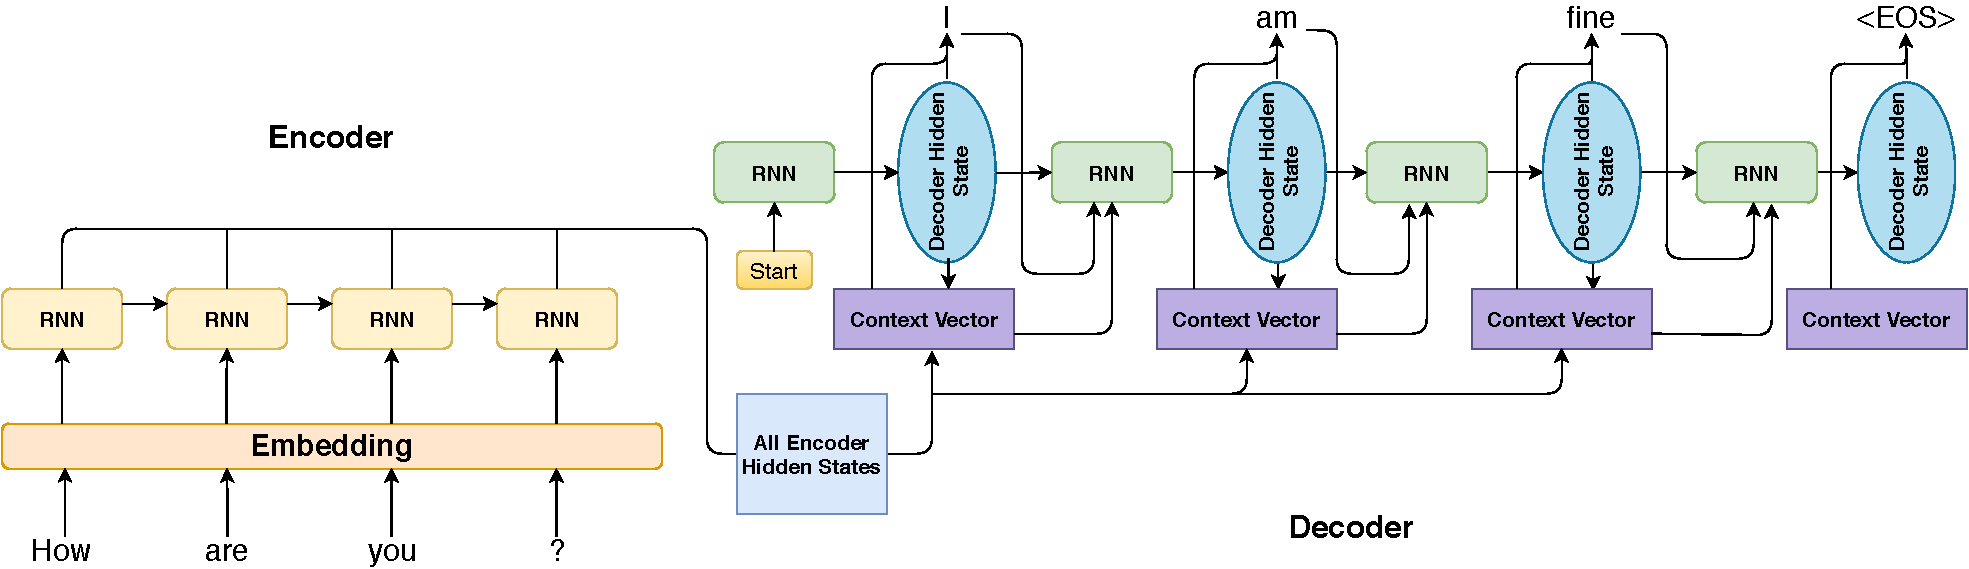
\includegraphics[width=1\textwidth]{figures/luong_decoder.pdf}
  \caption{Luong decoder architecture.}
  \label{luong}
\end{figure}

Luong attention model is classified into 2 categories, \textit{global} and \textit{local}. Common to these types of model is the fact that at each time step \textit{t} in the decoding phase previous hidden state is taken as input to derive a context vector $\mathbf{c_t}$, that captures relevant information to predict the current target word $y_t$. This categories differ only if ``attention'' is placed on all source positions or on a few source positions.

The simple concatenation layer combines the information from vectors $h_t$ and $c_t$ to produce an attentional hidden state (Equation \ref{eq:hs}).
\begin{equation} \label{eq:hs}
\mathbf{\widetilde{h_t}} = tanh(\mathbf{W_c}[\mathbf{c_t};\mathbf{h_t}])
\end{equation}

The attention vector $\mathbf{\widetilde{h_t}}$ then passed through the softmax layer to produce the predictive distribution (Equation \ref{eq:sfm}).
\begin{equation} \label{eq:sfm}
p(y_t|y_{<t},x) = softmax(\mathbf{W_s}\mathbf{\widetilde{h_t}})
\end{equation}

\subsubsection{Global Attention}
An alignment vector $a_t$ (size of $a_t$ is equal to the number of time steps on the source side) is derived by comparing the current target hidden state $\mathbf{h_t}$ with each source hidden state $\mathbf{\bar{h}_s}$ (Equation \ref{eq:av}).
\begin{equation} \label{eq:av}
a_t(s) = align(\mathbf{h_t}, \mathbf{\bar{h}_s}) = \frac{exp(score(\mathbf{h_t}, \mathbf{\bar{h}_s}))}{\sum_{s'} exp(score(\mathbf{h_t}, \mathbf{\bar{h}_s}))}
\end{equation}

There are three types of the score function (the score function is referred as a content-based function) (Equation \ref{eq:sf}).
\begin{equation}\label{eq:sf}
score(\mathbf{h_t}, \mathbf{\bar{h}_s}) = \begin{cases} \mathbf{h_t}^\intercal \mathbf{\bar{h}_s}, & \mbox{dot} \\ \mathbf{h_t}^\intercal \mathbf{W_a} \mathbf{\bar{h}_s}, & \mbox{general} \\ \mathbf{v_a}^\intercal tanh(\mathbf{W_a} [\mathbf{h_t}; \mathbf{\bar{h}_s}]), & \mbox{concat} \end{cases}
\end{equation}

In location-based function the alignment scores are computed from solely the target hidden state $\mathbf{h_t}$ (Equation \ref{eq:sfm_as}).
\begin{equation} \label{eq:sfm_as}
a_t = softmax(\mathbf{W_a}\mathbf{h_t})
\end{equation}

The context vector $\mathbf{c_t}$ is computed as the weighted average over all the source hidden state, where alignment vector represents weights.

\subsubsection{Local Attention}
Global attention is expensive, because it has to attend to all words on the source side for each target word. Local attention chooses to focus only on a small subset of the source positions per target word.

The local alignment vector $a_t$ in this category of attention is fixed-dimensional, because of it there are 2 variants of the model, \textit{monotonic} (Equation \ref{eq:monotonic}) and \textit{predictive} (Equation \ref{eq:predictive}).

\begin{equation} \label{eq:monotonic}
p_t = t
\end{equation}

\begin{equation} \label{eq:predictive}
p_t = S \cdot sigmoid(\mathbf{v_p}^\intercal tanh(\mathbf{W_p} \mathbf{h_t}))
\end{equation}

In monotonic alignment the source and target sequences are roughly monotonically aligned. In predictive alignment the model learns to predict the alignment position, where $\mathbf{W_p}$ and $\mathbf{v_p}$ are the learned model parameters.

Gaussian distribution centered in $p_t$ is used to favor alignment points near $p_t$ (Equation \ref{eq:align_gaus}).
\begin{equation} \label{eq:align_gaus}
a_t(s) = align(\mathbf{h_t}, \mathbf{\bar{h}_s}) exp(-\frac{(s-p_t)^2}{2\sigma^2})
\end{equation}

